% !TEX root = ../thesis.tex
\chapter{A Framework for Simulating and Analysing Cyber-Physical Systems}
\label{chap:framework}
% Describe what better CPS tools would provide - environmental simulation, trained environment models, virtual environments, cross-environment simulation
% Despite the growth in interest in the fields of sensor networks, cyber-physical computing and the Internet of Things, developing and testing sensor networks remains a difficult task, requiring developers to build reliable software which interacts as expected with the environment it inhabits.



% Testing and understanding how the environment interacts with a sensor network and vice-versa relies on placing the devices in the target environment and waiting for/creating the desired phenomena to interact with the network. Phenomena can include events such as movement of devices/objects, passive or active interaction with people (pressing buttons, triggering motion sensors), or other sensor events. Performing test deployments can be expensive, time-consuming and difficult.

% Existing tools and techniques aren't adequate for reliably and comprehensively testing these devices in the context of their target environment and the phenomena which may occur within it. Existing approaches for testing sensor networks have focused heavily on accurately simulating devices, the network and power consumption, with great success \cite{cooja, tossim}. However,  support for interacting with the environment is limited, typically performed using recorded or designed sensor trace data. This approach can be inaccurate, unrealistic and is restricted to what was recorded.


Despite the distributed and physical nature of cyber-physical systems and the Internet of Things, tools and techniques to support the needs of their development have not evolved to support efficient and reliable testing in the context of the deployment environment. Many tools exist which support individual aspects of testing and development, however, each one is siloed from the rest, limiting a developer's capability and coverage of testing.

This chapter presents a CPS co-simulation framework designed to unearth tools from their silos to create a flexible, extensible and powerful co-simulation platform to close the cyber-physical loop in CPS development, simulation, testing and analysis. Treating the physical environment as a first class citizen, the framework makes it possible for developers to simulate and test CPS within a 3D virtual environment, pre-deployment. A CPS interacts with and is directly affected by its target environment and inhabitants within it. The framework makes it easier for developers to test and analyse CPS which rely upon human mobility and device placement.

The following sections in this chapter outline a set of requirements \ref{sec:requirements} for the framework, a distributed design for building a co-simulation platform supporting plug-and-play of multiple tools, including a sensor network simulator and 3D game engine.


% Drill down into the perfect or ideal scenario, what we want to be able to do
% Sell each requirement, as if it is paramount
% Space(Placement), Time(control), People(Mobility)
\section{The Ideal Framework: Primary Requirements}
\label{sec:Requirements}
This section describes a key set of requirements that are necessary for a framework to support simulating and testing cyber-physical systems in virtual environments not only comprehensively and accurately, but also efficiently and effectively, such that developers benefit from using such a tool over simply testing in the real world or in a sensor network simulator.

Each of these requirements focus on key aspects needed for the framework to be effective for testing cyber-physical systems, which are deeply integrated into our physical world.



\subsection{Phenomena-on-demand}
\label{sub:requirements_Phenomena-on-demand}
In order to test a CPS in the real-world, developers often need to wait for or force desired phenomena to occur in order to observe how the system reacts and whether or not it reacts correctly. However, exercising control over the real-world is a difficult and time-consuming challenge. Similarly, enlisting human participants to perform repetitive, mundane tasks requires paperwork, significant time and often money. Lastly, some scenarios are simply not feasible to test due to their scale, limited access to a deployment environment or health and safety concerns, e.g., peak office hours, outdoor environments, evacuation, fire, flooding.

Ideally, the framework should provide a realistic and real-time physics engine to create dynamic, controllable and flexible phenomena which interact with the cyber-physical system on-demand. Phenomena could be created through either direct control, in which a developer directly interacts with the simulation by taking control of an entity or agent; or scripts. For example a developer could instruct agents to navigate along a path a set intervals to a meeting point, directly pick up and move a node, or trigger a fire to start and spread along a set of rooms via a common corridor. Each of these phenomena will dynamically generate physics events that can trigger sensors within a CPS.

Unlike traces, a scripted phenomena, such as a moving object, mobile node or person walking down a corridor, dynamically generates sensor input in real-time as it moves. Thus, only the phenomena script needs to be updated to change its path or behaviour; whereas, developers must update multiple traces, feeding sensors simulated ``detections'' inputs, for each sensor device in the entity's path, a time-consuming and unscalable solution.


\subsection{Human Mobility} % (fold)
\label{sub:requirements_mobility}
Existing tools support the concept of device mobility, updating a device's radio model based on its location. However, in these tools device mobility is static and pre-determined; in other words, developers define mobility patterns, as a sequence of positions, manually, which the network of devices must follow, but does not react to the live cyber-physical simulation. The tools have no concept of other entities, such as people, physical objects or gravity.

The tools lack of support for simulating human mobility, such that developers are required to manually trigger sensors or create custom scripts which attempt to model the mobility for each test scenario, in which the script triggers button presses or motion sensors at specified time intervals. As the network grows, shrinks or the layout changes, developers need to update the model for each device; this quickly becomes unmanageable as the network and number of tests scale in size.

Ideally, the framework should support testing CPS utilising real-time dynamic and reactive human (and device) mobility, enabling simulations to support testing environments in which virtual human participants interact with and are affected by the CPS and the environment, closing the cyber-physical loop. In other words, virtual participants are able to autonomously navigate an environment, based on flexible pre-assigned behaviours; including simple actions, such as patrol this corridor or walk to location A; or more complex behaviours, such as follow or avoid person X, wait on an event before moving. Whilst target locations may be pre-defined, routes may change in real-time based on obstacles or other behaviours. By combining behaviours, participants can dynamically generate phenomena in real-time for the CPS to sense and react to, without the need to edit scripts or manually interact with the system, even as it grows, shrinks or changes in layout. Participants are also reactive to changes caused by the CPS, such as closing a door, forcing the participants to navigate around obstacles or change their behaviour. 

Using such a system, when simulating a fire evacuation scenario, participants dynamically react to fire avoiding it as it spreads throughout the environment, with the CPS able to sense, alert and direct evacuees towards safe exits.

In various scenarios, including people during an evacuation, the concept of physiological and cognitive attributes can also have a significant impact when simulating human mobility behaviour\cite{Johnson2008}, such as age, fitness, assertiveness, risk-aversion, panic and fear\cite{TCPP_Personality_Profile}. Age and fitness of an agent can dictate their speed and vulnerability during an escape, causing them to slow down if there are old, unfit, injured or have a disability. Cognitive attributes, such as assertiveness or aggressiveness may cause them to charge through a path, forcing others out the way, or they may form or influence a herd. Alternatively, risk-aversion, panic and fear may cause agents to ignore evacuation signs, stay put or egress via the entrance they entered the building, even when passing sign-posted exits that offer a more rapid evacuation\cite{Johnson2008,Helbing,Sime1983}. Relationships can also have an affect on the evacuation speed of occupants: as parents wait or search for children, slowing down their escape and blocking others; or a group of friends or colleagues attempt to form before evacuating an area, again slowing themselves and other down.


\subsection{Placement}
\label{sub:requirements_3D design and placement}
The issue of placement in CPS is tightly coupled to provisioning, i.e., what is the minimum number of devices needed and where should these devices then be placed in order to achieve the desired coverage, reliability, or other desired metric. 
Understanding how many devices are needed for a specific deployment and where to place them within the environment is a difficult challenge pre-deployment. Often based on guess-work, trial-and-error and field studies, which can lead to both over- and under-provisioning, resulting in either high-cost, a lack of network reliability, insufficient or redundant sensor data, etc. 
Thus, virtually experimenting with placement ahead of time will help mitigate these issues before deployment. 

Testing different placement strategies within a 3D virtual world would enable developers to quickly move nodes around an environment programmatically or by visually dropping them into place, without the need to manually change scripts and sensor input traces; instead, the virtual world dynamically generates sensor inputs in real-time for nodes based on their new positions. Similarly, developers should be able to flexibly scale the levels of device provision, to test and understand how it will affect a deployment. 

Ideally, the system should support automatically testing and suggestion of optimum placement and provisioning levels, based on selected criterion, such as cost, quality-of-service, robustness, coverage, etc.

%%%%%%%%%%%%%%%%%%%%


% subsection mobility (end)


% Using Ard\'{a}n, developers can take direct control of a virtual person or script intelligent virtual crowds to carry out tasks, such as walking between points, avoidance, following or interacting with objects. Figure \ref{fig:views} shows people walking up and down a corridor, avoiding each other's path. Unlike using trace data, genuine or created, developers can easily tweak scenarios, such as moving sensors, people or adjusting behaviour, to test subtle or significant variations. Developers can also create scenarios that are difficult or dangerous to reproduce in the real world, such as emergency situations, and repeatedly test their applications without risk.

\subsection{Time Control}
\label{sub:requirements_Time Control}
In real-world deployments developers have no control over time and have to analyse events as they happen or rely on logs and video to record and view post-test. Simulation approaches enable pausing and slowing time, giving developers more time to analyse snapshots or small windows of time in a test, however, recording still utilises log-based approaches, providing only a limited snapshot. Both approaches provide limited views into a test, if events were not recorded, via logs, video or otherwise, they are lost and the test must be re-run.

Recording everything would enable a simulator to create a full reconstruction and allow developers to master time-control, moving forwards and backwards through a simulation to view its state at any point in time. Within a 3D environment, this would also allow developers to observe the context in which particular phenomena occur, enabling in-depth and contextual analysis.

Naturally, the system should support recording arbitrarily long, such as day- or even week-long, simulations, enabling longitudinal testing of CPS applications in real-time or faster. The system must also provide the means to quickly scrobble through recordings, based on time or checkpoints, generated based on points of interest, e.g., when a network partition occurs.


% subsection distributed (end)
% Unlike in real world deployments, developers have the power to control time in the simulated world. Developers can: stop-the-clock, freezing both the simulation and world in time, whilst giving them full control over what they see, allowing more time to observe the environment and move between points of interest; slow down time, giving developers more time to observe or control the simulation; or even speed up time, providing desired results in considerably less time.


\subsection{Visualisation - Visual Diffing and Analytics}
\label{sub:requirements_Visualisation}
To complement log output, existing CPS simulators provide basic 2D visualisations, such as 2-dimensional network maps and transmission timelines\cite{cooja_timeline,NS2}, giving developers more insight into the network component in real-time. However, visualisation development has only focussed networking information, with other information only presented in logs or tables. Visualisations in existing tools are ephemeral and can only be viewed once as the simulation is on-going, anything missed is lost and the simulation restarted. Visualisations can be recorded, however, once recorded to video the visualisations can no longer be explored and investigated for in-depth info. If a developer wants to compare two separate simulation runs, they must resort to post-simulation log analysis, typically using external tools to manually process the log output into another form, visual or otherwise, without the context of the simulator visualisation tools.

Firstly, visualisations should provide visual context to developers both during and after a simulation, with the capability to explore and investigate previously unseen data or snapshots, thus, simulators or the visualisation tools must record generated visualisation data in a replayable format.

Secondly, visualisations should not just help developers understand a single simulation but should also help developers to spot and analyse differences, ``visual diffing'', between multiple simulation runs in real-time, without the need the need to leave the tool to perform post-simulation data analysis using manual tools. When simulating in a 3D virtual world, visual diffing will empower developers to see, explore and analyse cyber-physical systems in the context of the virtual world and past simulation runs.

However, when simulating in the context of a 3D virtual world, visualisations must add value to already busy simulations, with the aim to reduce the visual noise, not add to it. Thus, visualisations should not simply be layered on top of the 3-dimensional virtual world, akin to a lap or split time on a racing video, instead they should seamlessly integrate into the virtual environment to provide intuitive visual feedback, indicating points of interest, such that they further enhance a developers analytical tool-kit and understanding of an on-going simulation. 


These visual differencing tools, would allow developers to specify events of interest to watch, which the simulator then visually flags to the user when it happens, e.g., a node glows red when it's power levels drop below a certain point, or differ from a previous simulation run by x\%. Similarly, visualisations should also support longitudinal studies of systems.
% Ard\'{a}n provides developers tools to overlay visualisations of network and sensor meta-information on top of the virtual world to help understand how the network is running, allowing developers to see information such as how network paths form as packets are sent, as well as transmissions, receptions, interruptions. In figure \ref{fig:views}, sending devices are highlighted with a circle and receiving devices are connected by an arrow to the sender, each device is represented with its own colour, to help differentiate simultaneous transmissions.

\subsection{Virtual Sensors and Actuators}
\label{sub:requirements_Virtual Sensors and Actuators}
Sensor and actuator devices have both a hardware and software representation, thus, a framework must reflect both of these components within the simulated world. The CPS simulator runs the device program code, simulating the CPU, network and other virtual components, whilst within the game engine the device has a physical form with sensors and actuators that can sense and interact with the virtual world. 

This will enable a co-simulation approach in which simulated hardware devices can interact directly with the 3D virtual environment, and not just with faked or simulated input from traces or user input. The framework will provide developers with flexible and dynamic environmental interaction between the CPS and the environment, closing the loop within a simulation. A device's sensors should be modelled using the framework's physics engine to provide dynamic and realistic sensor feedback, reacting to phenomena in the 3D virtual environment in real-time. Similarly, actuators should enable devices to physically interact with the virtual environment to close the cyber-physical loop in simulation e.g., opening a door, turning on a light, or sounding an alarm. Alternatively, it is not necessary for devices to match or be constrained by their real-world counter-parts, thus, sensors may be modelled more accurately or powerful, enabling them to sense faster, with greater range or more fidelity; or less accurately depending on the testing scenario needs and the simulation performance available.

Visually, device hardware can be modelled at varying degrees of accuracy, depending on the requirements, e.g., virtual devices can be larger in size compared to real counter-parts, enabling easier location and observation. Similarly, sensing can be simulated to varying degrees of accuracy, again depending on the needs and simulation power available. 

% Within Ard\'{a}n we have modeled several basic sensors and actuators, including motion detectors, buttons, lights and location. These act as virtual hardware for the simulated sensors, allowing the simulation to interact with the virtual world. Virtual sensors can be designed to model a real sensors behaviour, or be virtually improved, providing higher accuracy or more features, not possible with existing hardware.

\section{Secondary Requirements} % (fold)
\label{sec:secondary_requirements}

% section secondary_requirements (end)

\subsection{Environment-based Radio Simulation} % (fold)
\label{sub:environment_based_radio_simulation}
Ideally the framework should allow for the export of the built 3D environment used for virtual deployments, to provide environment-based radio simulations tools the same 3D environment model for generating a realistic radio model. Using the exported 3D model, the radio simulator could generate a realistic radio model based on the physical environment, such as walls, objects and other structures, and its attributes, such a material type, thickness, orientation, reflectivity.\cite{trunetWireless}

% subsection environment_based_radio_simulation (end)
\subsection{Distributed component-based simulation} % (fold)
\label{sub:distributed}
The co-simulator should be discretised into components with clear interfaces; such that the architecture allows for distributing components across multiple machines. Similarly, the architecture should support for allowing virtual components to be swapped out for other components, or their real counterparts e.g., swapping out a set of virtual simulated nodes for a set of real deployed hardware nodes. Enabling developers to test real vs. simulated nodes and potentially visually diff them to further analyse their differences.

\subsection{Extensibility} % (fold)
\label{sub:requirements_extensibility}
The framework design should facilitate seamless integration of new tools to supplement or replace the existing ones. This allows future developers to build upon and improve the co-simulation framework, its output and experience through the use of additional tools, including simulation tools, analytical tools, model checkers or real test-beds.

\subsection{Direct control}
\label{sub:requirements_direct_control}
The framework should allow direct control of three key aspects of the simulation: entities in the world, such as environmental attributes and physical devices or sensors; virtual people in the 3D world, enabling the developer to inhabit the world vicariously through a virtual person, interacting and responding to the world as if it were the real world; lastly, the view, allowing the developer to view the world from any angle at any point in time, including pausing the world mid-simulation and moving around, providing a better view of a point of interest.

\subsection{Write Once, Test Everywhere}
\label{sub:requirements_real_code}
Using a single language for both testing and deployment, in the real- and virtual-world, significantly reduces the time and effort for transferring between the different environments and ensures a consistent code-base, with the hope for consistent performance and output. Similarly, using an existing language reduces barrier to entry for use of a new tool and eliminates the opportunity for translation bugs being introduced when transitioning between test and deployment, whether they be real or virtual environments.

\subsection{Performance}
\label{sub:requirements_real-time_operation}
The system should support real-time operation so that simulations run as fast as, if not faster than their real counterparts, enabling quicker deploy-test-debug cycles. Similarly, it needs to be responsive to real-time direct interaction by developers, such that developers can observer, interact with and change ongoing simulations. Thus, in order for the framework to run in real-time, each of the components must also run accordingly. In order for the sensor network simulator to run in real-time, the 3D game engine must respond to all requests in real-time (sensor reads), such that the virtual hardware is in-discernible from the real counterpart.

\subsection{Synchronisation}
\label{sub:requirements_synchronisation}
Synchronisation, between the various components, including CPS simulator and 3D game engine clocks, ensures time sensitive events which rely on a global notion of time and delays occur correctly. Whilst real-time operation is also a requirement for all sub-systems, due to the differing simulation methods which aren't 100\% accurate and the intricacies of OS level scheduling, synchronisation is necessary to ensure that the individual sub-system's clocks stay in sync, within reasonable bounds. Similarly, communications between the sub-systems must be of low enough latency such that no additional delays are introduced. Typical applications are designed with predictable or known delays, such as opening a door after a motion event.

\subsection{Test cases}
\label{sub:requirements_test_cases} 
The system should provide support for automated testing, to observe and assert conditions about not only the CPS, but also the virtual world environment, akin to unit-testing available in traditional application development. Assertions would provide developers with warnings about phenomena that have occurred on a particular node, area, or within entire environment, such as ensuring a light's duty cycle doesn't exceed a set limit, checking a group of nodes are reporting similar information, or checking for network partitions once a node has moved out of an area.


\subsection{Modular environment building}
\label{sub:requirements_modular_building}
Designing 3D environments from scratch can be a slow and difficult process for non-expert 3D designers such as developers. Thus, in order to enable fast set-up, the system must support re-use and modification of existing pre-built environments and provide modular building blocks for building environments e.g., walls, doors, rooms, sensors, lights, agents.


% MOTHERHOODS - Scalable, extensibles, blah
\subsection{Scalability} % (fold)
\label{sub:requirements_scalability}
The scale of cyber physical systems can range significantly between self-contained deployments within a single room to ones which cover entire buildings, streets or even cities. Deployments could be internal, external or a mix, each of which may effect design decisions and issues that may arise. A simulation framework needs to be capable of supporting from 10s to 100s of devices. Similarly, the simulator must also be able to support rich environments, including complex layouts, large numbers of people to inhabit the world and environmental effects.
% subsection scalability (end)



% % subsection extensibility (end)
% \textbf{Common Schema - }
% In order to ensure information communicated between individual sub-systems correspond, all information passed between the different tools must match or conform to a common schema, such as time, location and sensed units; without this conformity, even the simplest of interactions, such as device movement through a space, could be misunderstood between sub-systems, cm vs mm vs feet. This builds upon the extensibility requirement, ensuring future tools that support the schema will integrate seamlessly into the system.





% \textbf{Time control - }
% Whilst observing an ongoing simulation the developer should be able to pause the ongoing simulation allowing them to view a snapshot in time in more detail, both in terms of the running application and the 3D world, before resuming, speeding up or stepping through the simulation. Full control would allow the developer to also rewind back to an earlier state in the simulation and 3D world, enabling the developer to replay a set of events and observe multiple points of interest from different angles.





% \textbf{Scripted control - }
% Automated test cases are an important tool for testing systems repeatedly, thus, to support this the tool should allow developers to create scripted scenarios, in which people and objects within the 3D world can be instructed to follow set actions based on events, be it time, key presses or world events.



\chapter{Framework}
\label{sec:framework}
The current state-of-the-art tools for cyber-physical systems focus on individual aspects of testing, such as network or hardware simulation, but are siloed from other tools. Many other tools and platforms exist that could support these CPS tools with other aspects of CPS testing, such as environment and physics simulation, formal modelling, or statistical analysis tools, without the need to directly extend or integrate these features within any of them. 

Hence, the goal of this framework is to provide an open, stable and extensible platform into which a variety of tools can be integrated to support the simulation, testing, modelling and analysis of cyber-physical systems.

This section proposes an architecture for designing a distributed framework supporting a co-simulation approach for testing and analysis of cyber-physical systems using multiple tools.
This will enhance the information sharing between tools, enabling developers to seamlessly use these tools in tandem and close the loop, e.g., 3D simulator updates positions of devices based on physical interaction with the virtual world, this is then reflected in the network simulator which affects the radio transmission range and interference.

\section{Architecture and Communication} % (fold)
\label{sub:architecture}
Rather than integrate different co-simulation components together directly, our approach uses a publish/subscribe event bus and common schema to describe information passed between the different tools. This approach reduces the tight coupling between tools, allowing for individual tools to be removed, added or replaced with minimal configuration. We envision the integration of tools such as model checking, statistical analysis, unit-testing and advanced simulation for radio and environmental properties.

Each tool publishes or subscribes to the relevant topics of interest within the event stream, enabling other tools to observe or inform one another of events in a many-to-many fashion. Typically, only one tool will publish data to a topic related to that which it specialises in, e.g., radio simulator publishes when transmissions were sent and received. Other tools subscribed to this stream may then publish a composite event, adding more data, analysis or context back to the event stream.

To support the platform each tool needs to build a plugin which communicates between the event bus and tool itself, subscribing to and publishing data. A tool's plugin defines a set of topics to which it publish/subscribe to, providing developers with a clear interface between co-operating tools.
% subsection architecture (end)
\begin{figure}[ht]
\centering
  % \includesvg[svgpath = ./imgs/, width = 0.5\textwidth]{architecture}
  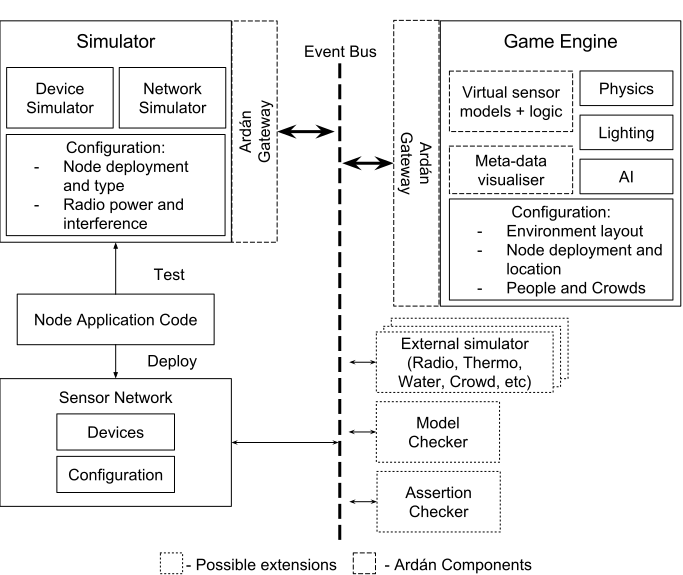
\includegraphics[width=\textwidth]{./imgs/architecture}
  \caption{Ard\'{a}n architecture}
  \label{fig:architecture}
\end{figure}



\section{Time} % (fold)
\label{sub:time}
Within the simulation world there are two clocks, the simulated time and the real world or wall clock time, how much time has passed in the simulation reality and how much time has passed the the real world. Comparing these two times gives us the simulation rate, i.e., how much simulated time passes in 1 second of real world time. It's often the case that simulations can run faster than real-time, resulting in a simulation rate >1x, providing results faster than had they been carried out in the real world. Similarly, users can also select to run simulations slower than real-time, giving developers more time to observe and analyse the simulation in real-time.

When performing co-simulation between different components or tools, it's necessary to ensure the simulation tools remain synchronised, such that the individual simulations aren't adversely affected, e.g., the CPS simulation lags behind the virtual world simulation, resulting in delayed and slow CPS response times, causing devices in the virtual world to actuate incorrectly.

Also, should a developer choose to run a simulation at a speed faster or slower than real-time, it is also necessary to ensure the co-simulation tools support this functionality and are instructed to simulate at the desired speed.
% subsection time (end)

\subsection{Human Mobility} % (fold)
\label{sub:human_mobility}
Within Ardan, the game engine component is responsible for human mobility, handling the physical modelling and characteristics, such as size, weight, speed and appearance, as well as their behaviours.

When creating a virtual person, henceforth referred to as a agent, developers can choose to create or spawn them in one of three ways: programmatically in C++, spawning an agent specifying their appearance, scale (size) and location; interactively, using the visual game engine editor to select a agent type, drag and then drop into the environment, before then assigning further attributes; scripting in the game engine's visual programming tool, similar to C++ in its API and programming logic, however, it provides developers with a visual drag-and-drop based programming tool, with useful auto-suggestions and completion.

Utilising the physics engine within the game, an agent's properties, such as size and weight, can have a significant impact on their interactivity with the world, such as their body fitting through spaces or their weight impacting their momentum and force in collisions with other objects. To navigate the physical environment, agents use a navigation mesh built by the physics engine, which calculates traversable paths for agents to use to navigate within the environment, around obstacles, through doorways and up ramps or stairs. Agents then use the A* algorithm on the navigation mesh to find the shortest path to their destination.

After spawning an agent, behaviours can be assigned to them which they will perform at run-time. Behaviours, similar to spawning an agent, can be created and customised using the previously mentioned methods. The visual programming tool simplifies this process, by enabling developers to interactively find and select entities of interest and create sequences of conditions and actions to form behaviours. Developers have access to a large API of primitives to support complex behaviours, such as sphere and ray tracing, used to detect and measure nearby and visible agents or entities. Behaviours can be as simple as move to a location, requiring an agent to navigate the environment and avoid any obstacles; or more complex, such as agent X follow agent Y, requiring the agent X to determine where Y is before than navigating to their position. 

Agents 

It is also possible to create crowd behaviours, such as herding, in which a group of agents move and perform actions as a collective unit, without any central decision making. These behaviours can be constructed by creating agent behaviours that are influenced by other agents and their behaviours. Within the game engine a  herd may start due to an agent following someone who they deem has authority in a situation (manager, teacher). The herd may also influence other agents to join in due size of the group, 'flocking'. For example, within a fire evacuation a manager may form a herd with colleagues leading them to a safe exit, other agents observing would choose to follow even if the route was neither the safest nor quickest.

Group behaviour, family/friends waiting/searching

Occupant aggression, physiological differences

% subsection human_mobility (end)